%
% Complete documentation on the extended LaTeX markup used for Insight
% documentation is available in ``Documenting Insight'', which is part
% of the standard documentation for Insight.  It may be found online
% at:
%
%     http://www.itk.org/

\documentclass{InsightArticle}


%%%%%%%%%%%%%%%%%%%%%%%%%%%%%%%%%%%%%%%%%%%%%%%%%%%%%%%%%%%%%%%%%%
%
%  hyperref should be the last package to be loaded.
%
%%%%%%%%%%%%%%%%%%%%%%%%%%%%%%%%%%%%%%%%%%%%%%%%%%%%%%%%%%%%%%%%%%
\usepackage[dvips,
bookmarks,
bookmarksopen,
backref,
colorlinks,linkcolor={blue},citecolor={blue},urlcolor={blue},
]{hyperref}
% to be able to use options in graphics
\usepackage{graphicx}
% for pseudo code
\usepackage{listings}
% subfigures
\usepackage{subfigure}


%  This is a template for Papers to the Insight Journal. 
%  It is comparable to a technical report format.

% The title should be descriptive enough for people to be able to find
% the relevant document. 
\title{Parallel algorithms for erosion and dilation of label images.}

\newcommand{\IJhandlerIDnumber}{3399}

% Increment the release number whenever significant changes are made.
% The author and/or editor can define 'significant' however they like.
\release{0.00}

% At minimum, give your name and an email address.  You can include a
% snail-mail address if you like.
\author{Richard Beare{$^1$} {\small and} Paul Jackway{$^2$}}
\authoraddress{Richard.Beare@monash.edu\\Department of Medicine\\Monash University\\Melbourne\\Australia{$^1$}\\CSIRO Mathematics Informatics and Statistics\\Dutton Park\\Queensland\\Australia{$^2$}}

\begin{document}

\IJhandlefooter{\IJhandlerIDnumber}

\maketitle

\ifhtml
\chapter*{Front Matter\label{front}}
\fi


\begin{abstract}
\noindent
It is sometimes useful to be able to apply binary morphological
operations, such as erosions and dilations, to labelled images in a
fashion that preserves the labels. This article introduces a
specialised class implementing parallel methods described in
\cite{beare2011parallel} that provide very fast dilations by circles
and spheres of arbitary size. Comparisons with other implementations
using currently available building blocks are also made.
\end{abstract}
\IJhandlenote{\IJhandlerIDnumber}
\tableofcontents

\section{Introduction}
The link between Euclidean distance transforms and binary
morphological operations is well known - erosions and dilations by
circles and spheres can be performed by thresholding the distance
transform. Efficient and readily parallelizable distance transform
algorithms can, in turn, be based on erosions and dilations by
parabolic structuring elements. The classes outlined in this article
extend the contact point algorithm used for parabolic erosions and
dilations to facilitate operations on label images. A more complete
discussion is available in \cite{beare2011parallel}. The classes
introduced here are able to separate touching labels during erosion
and split touching labels at the midpoint during dilation.

\section{The classes}
The {\em itk::LabelSetDilateImageFilter} and {\em
  itk::LabelSetErodeImageFilter} implement dilation and erosion of
label images. They share a common parent class. The methods controlling class behaviour are:
\begin{itemize}
\item {\em UseImageSpacing}: Defines whether the radius refers to voxels or world dimensions. Default is false, meaning radius is in voxels.
\item {\em Set/GetRadius}: Set the size of the dilation or erosion. There are versions to set the size in all directions to be the same, corresponding to a circular or spherical structuring element, and independently, corresponding to an ellipsoid structuring element (with axes parallel to image axes).
\end{itemize}

Examples of use are available with the package.

Please note that these are specialised classes which cannot use
arbitrary structuring elements.

The code from this contribution is also available at
\url{https://github.com/richardbeare/LabelErodeDilate}.

\subsection{Notes for label erosion}
The class provided for label erosion {\bf will separate} touching
labels. If this is not the desired behaviour, then implement label
erosion via binary erosion and masking.

\section{Alternative approaches to label dilation}
As advised on the ITK mailing list, label dilation can be implemented
via distance transforms and watershed transforms. This algorith is
illustrated in SimpleITK python code below (courtesy of Bradely
Lowekamp):

\lstset{language=Python}
\begin{lstlisting}
def MultilabelDilation(img, radius=1,kernel=sitk.BinaryDilateImageFilter.Ball):
    distImg = sitk.SignedMaurerDistanceMap(img != 0,
                                           insideIsPositive=False, 
                                           squaredDistance=False, 
                                           useImageSpacing=False)
    dilatImg = sitk.BinaryDilate(img!=0, radius, kernel)
    wsImg = sitk.MorphologicalWatershedFromMarkers(distImg, img)
    return dilatImg*wsImg
\end{lstlisting}

There are a couple of altnernatives to this algorithm implemented in
C++ and provided in {\em multilabelDilation.h}. The first version is a
variant of the code above, which avoids using the binary dilate
operation and thresholds the distance transform instead. This version
is called {\em multilabelDilation}. The second version uses the {\em
DanielssonDistanceMapImageFilter} to produce both a distance map and a
Voronoi tesselation. The distance map is thresholded to produce a
dilation which is then used to mask the Voronoi tesselation. This
version is called {\em multilabelDilationDanielsson}. The Danielsson
filter is slower than the Maurer filter, but this approach avoids the
watershed transform step as the information provided by the Voronoi
map is removes the need for the watershed. Comparisons of performance
are below.

\subsection{Problems with the watershed approach}
It turns out that the distance transform followed by watershed
transform approach to label dilation only works reliably for smaller
dilations, say 10. For larger dilations there is a chance of regions
leaking across borders and becoming incorrect. Leaks of this kind
result from the nature of propagation in the border zone combined with
tied distance values. 

\subsection{Dilations via distance maps versus binary dilation}
There are subtle differences between the effective structuring element
produced when thresholding distance maps versus those provided by the
{\em BinaryBallStructuringElement}. The latter is a Bresenham circle
or sphere, which means that any voxel which is partly inside the
specified radius is included in the structuring elements. Distance
maps, on the other hand, typically compute distances to voxel
centres. Thus any voxel whos centre is closer than the specified
radius is included, resulting in a slightly smaller structuring
element. 

In addition, the parabolic dilation used in the LabelDilate tool
treats voxels with centres exactly the dilation radius from the seed
as ``outside''. This results from the optimized use of the contact
point algorithm to avoid computation of a complete distance
transform. There may be some fudge factors that can be added to avoid
this behaviour, which will be investigated in the future.

\subsection{Other differences}
There are minor differences in results obtained from the Danielsson
approach and the new approach discussed here. Some of those
differences are along boundaries. My investigations suggest that the
Danielsson approach is wrong in these cases. Explicit calculation of
the distance between the locations of seeds and differences in
labelling indicate that the points are incorrectly labelled by the
Danielsson approach. The {\em reportNonZero} tool and {\em check.R}
functions were used to investigate these problems.

\section{Performance}
The specialised version was developed due to ease of parallel
implementation and performance results show that it is indeed much
faster than versions that can be built using existing tools. It also
scales moderately well with increased execution threads. The execution
times and speedups for a 12 core Intel(R) Xeon(R) CPU X5650 @ 2.67GHz
on a $182 \times 218 \times 182$ brain atlas are shown in Figures
\ref{fig:exec}. None of the methods have a
significant dependence on dilation size, as the structuring element is
not explicit. Speedup at 8 cores for the Maurer method is 1.86
versus 4.71 for the parabolic method. The lack of scalability of the
Maurer method is likely to be largely caused by the watershed step,
which is not parallel. The Danielsson approach is much slower, despite
avoiding the need for an explicit watershed transform. There is some
redundancy in the Maurer approach, as a signed distance transform is
computed by not used. In the single threaded the specialised version
is 7 times faster than the Mauer approach and 180 times faster than
the Danielsson-based method.

\begin{figure}[htbp]
\centering
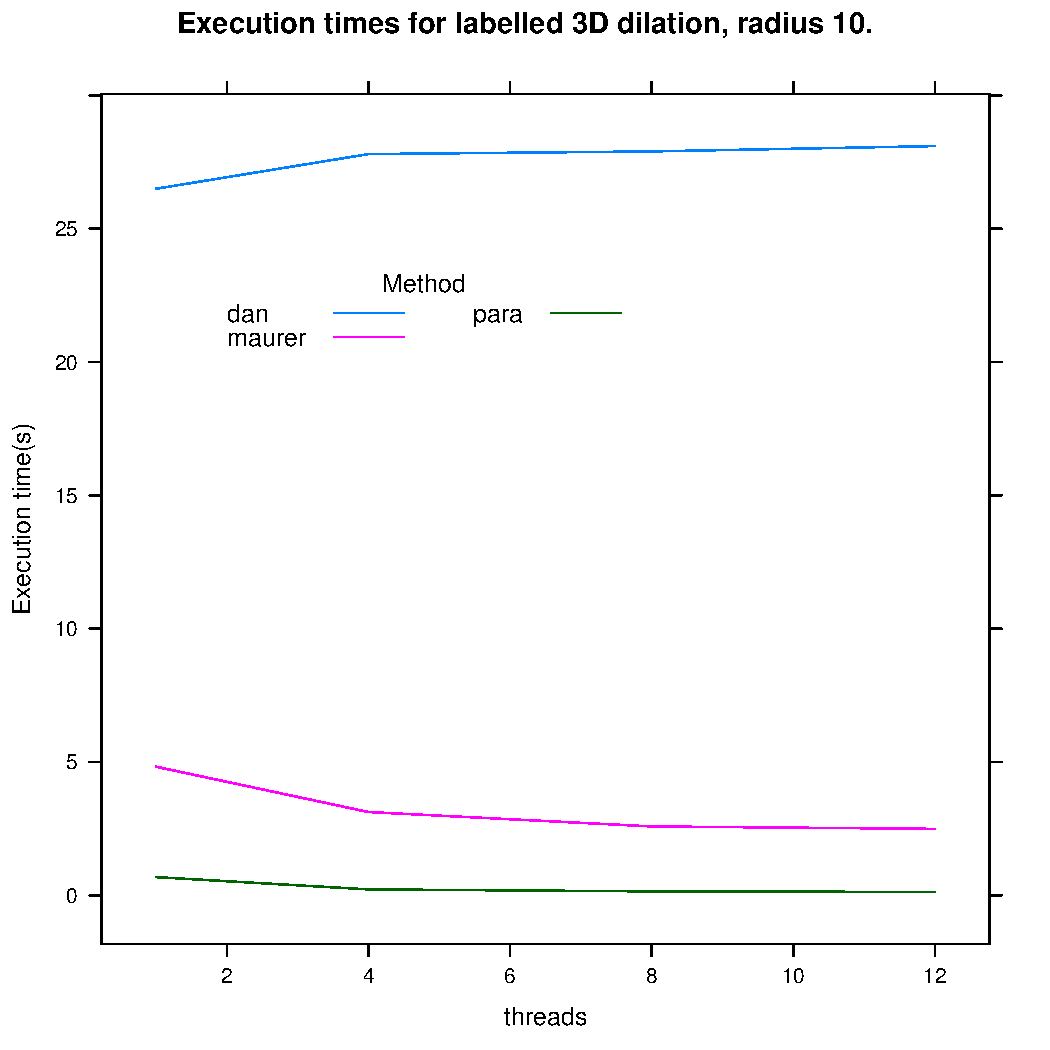
\includegraphics[scale=0.35]{exectimes}
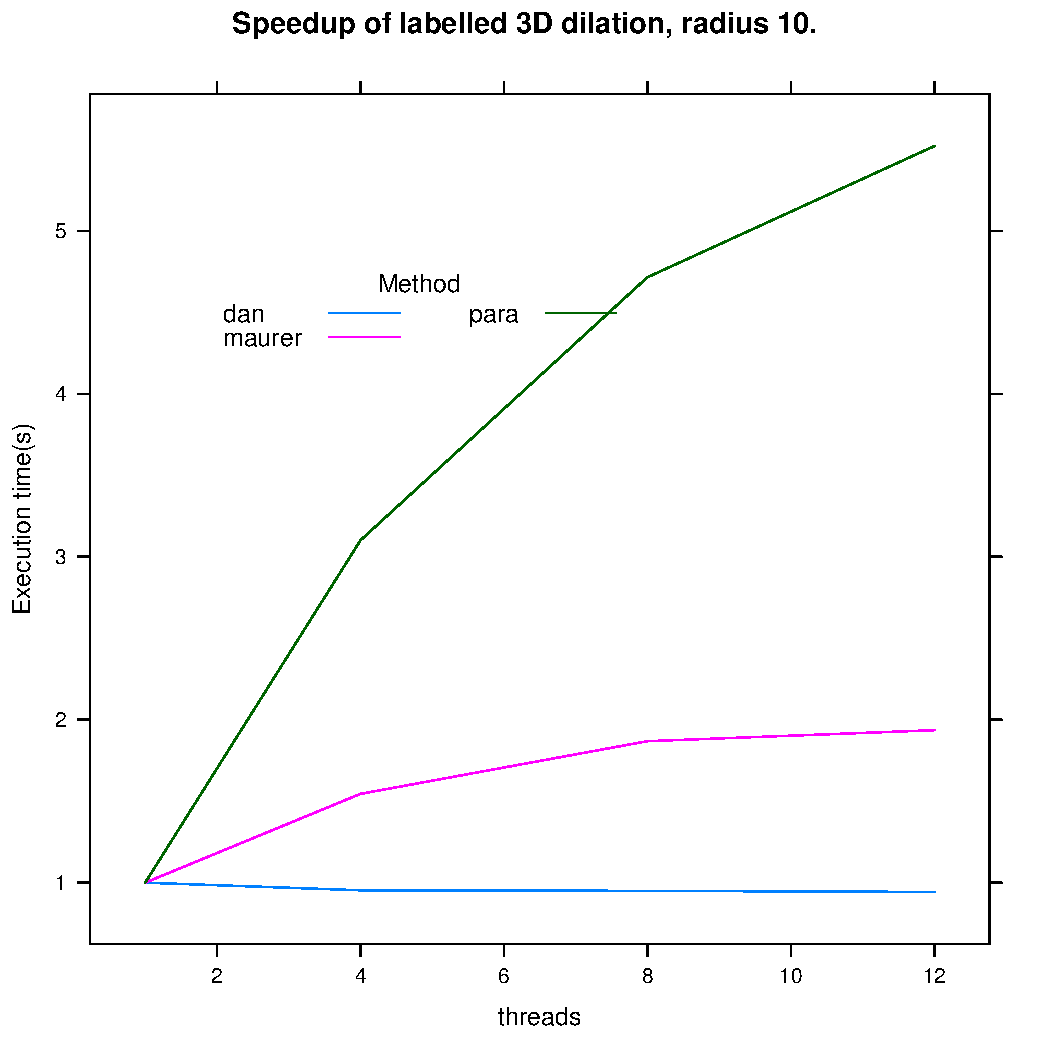
\includegraphics[scale=0.35]{speedups}
\caption{Execution times and speedups for all methods.\label{fig:exec}}
\end{figure}


\section{Sample results}
Label images occur in many situations. This is an example of a brain
atlas in which different labels represent different anatomical
regions. Examples of 2D processing (operations applied to a single
slice of the atlas) are shown in Figure \ref{fig:2d}. Examples of a 3D
processing are shown in Figures \ref{fig:3dorig} to \ref{fig:3ddil}.

\begin{figure}[htbp]
\centering
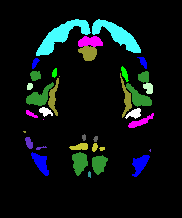
\includegraphics[scale=0.75]{axial_color}
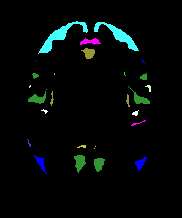
\includegraphics[scale=0.75]{laberode2d_color}
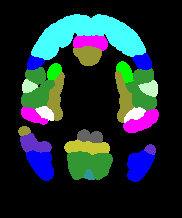
\includegraphics[scale=0.75]{labdilate2d_color}
\caption{Original, eroded and dilated atlases - a single slice with a 2d circular structuring element.\label{fig:2d}}
\end{figure}

\begin{figure}[htbp]
\centering
\includegraphics[scale=0.15]{atlas_orig}
\caption{Axial, sagittal and coronal slices through a labelled brain atlas.\label{fig:3dorig}}
\end{figure}

\begin{figure}[htbp]
\centering
\includegraphics[scale=0.15]{atlas_erode_color}
\caption{Atlas in Figure \ref{fig:3dorig} after applying 3d labelled erosion. \label{fig:3dero}}
\end{figure}

\begin{figure}[htbp]
\centering
\includegraphics[scale=0.15]{atlas_dilate_color}
\caption{Atlas in Figure \ref{fig:3dorig} after applying 3d labelled dilation. \label{fig:3ddil}}
\end{figure}



\section{Conclusion}
This article provides two classes for erosions and dilations of label
images using algorithms developed in a previously published
work. These methods use parallel, scan-line base algorithms that offer
very fast operations.
\bibliographystyle{plain}
\bibliography{local,InsightJournal}
\nocite{ITKSoftwareGuide}

\end{document}

